\documentclass[conference]{IEEEtran}
\IEEEoverridecommandlockouts

\usepackage[T1]{fontenc}
\usepackage[utf8]{inputenc}
\usepackage{cite}
\usepackage{amsmath,amssymb,amsfonts}
\usepackage{graphicx}
\usepackage{booktabs}
\usepackage{multirow}
\usepackage{url}
\usepackage{array}
\usepackage{xcolor}
\usepackage{tikz}
\usetikzlibrary{shapes.geometric, arrows.meta, positioning, fit, backgrounds, calc}

\title{Skillence: A Full-Stack AI Platform for Career Recommendation,\\
Market Intelligence, and Campus Placement Automation}

\author{
\IEEEauthorblockN{
Namit Rustagi\IEEEauthorrefmark{1} \quad
Rahul Gehlot\IEEEauthorrefmark{1} \quad
Manansinh Sandhaliya\IEEEauthorrefmark{1}
}
\IEEEauthorblockN{
Rajeev Ranjan Pratap Singh\IEEEauthorrefmark{1} \quad
Kshitiz Srivastava\IEEEauthorrefmark{1} \quad
Dr.\ Velmani Ramasamy\IEEEauthorrefmark{2}
}

\vspace{4pt}

\IEEEauthorblockA{\IEEEauthorrefmark{1}
Department of Computer Science and Engineering\\
VIT Bhopal University, Madhya Pradesh, India\\
namitrustagi11@gmail.com\\
rahulgehlot6044@gmail.com\\
sandhaliya1@gmail.com\\
rajeevranjanpratapsinghj94@gmail.com\\
kshitizsrivastava.india@gmail.com
}

\vspace{2pt}

\IEEEauthorblockA{\IEEEauthorrefmark{2}
Supervisor, Department of Computer Science and Engineering\\
VIT Bhopal University, Madhya Pradesh, India\\
velmani@vitbhopal.ac.in
}
}

\begin{document}
\maketitle

%% ---------------------------------------------------------------
\begin{abstract}
Career planning tools for university students are often fragmented across standalone resume builders, job portals, and placement systems, leading to redundant data management and inconsistencies between candidate profiles and opportunity matching. This paper presents Skillence, a unified career intelligence platform that integrates resume understanding, AI-assisted career-path recommendation, job-market analytics, salary prediction, skill development, and campus placement automation within a single system. The platform leverages document intelligence techniques for structured resume extraction and employs semantic ranking methods for aligning user profiles with relevant career opportunities. Machine learning models are trained offline and optimized for efficient, low-latency inference in production environments. The system operates on a large-scale dataset comprising approximately 30,000 job postings, 894 occupational roles, and a structured skill vocabulary, enabling data-driven recommendations and insights. Experimental evaluation shows that the salary prediction module achieves strong performance (R\textsuperscript{2} = 0.7258), outperforming a linear regression baseline (R\textsuperscript{2} = 0.5812), while maintaining inference latency of 50--100 ms. Additionally, the multi-stage recommendation pipeline improves computational efficiency by reducing unnecessary large-scale ranking overhead, and the placement matching module generates transparent, auditable results through component-level score decomposition. A pilot deployment demonstrates the system’s ability to maintain consistency across modules and support end-to-end career planning, from profile analysis to placement outcomes. The proposed approach highlights the effectiveness of integrating AI-driven components into a unified platform to enhance scalability, transparency, and efficiency in university placement ecosystems.
\end{abstract}

\begin{IEEEkeywords}
career intelligence, career recommendation systems, skill gap analysis, salary prediction, job market analytics, campus placement, machine learning, semantic ranking
\end{IEEEkeywords}

%% ---------------------------------------------------------------
\section{Introduction}

Career planning for university students involves at least four distinct
activities: understanding personal skill profiles, mapping those
profiles to realistic career options, interpreting labor-market demand
signals, and navigating campus placement processes. In practice, each
activity is served by separate tools that share no common data model.
Students must re-enter skills for resume parsers, job-matching engines,
and placement portals independently, and often receive contradictory
guidance across these surfaces. Placement cell administrators must
reconcile manually maintained spreadsheets with employer job
descriptions (JDs), introduce subjective criteria, and manage
shortlisting outside any systematic scoring framework.

Skillence is designed around the hypothesis that integrating these
activities within a single data model --- where a parsed resume flows
directly into recommendations, learning roadmaps, market analytics, and
placement scoring --- reduces friction for students and increases
transparency for administrators. The core design principle is
\emph{hybrid intelligence}: deterministic modules handle
policy-sensitive, auditable decisions (eligibility gating, weighted
scoring, shortlist ranking), while large language models (LLMs) are
used selectively where semantic synthesis is genuinely valuable
(ranking explanations, learning roadmap generation, market insight
narration). This strategy preserves explainability where it matters
most while retaining the flexibility of generative reasoning for
narrative tasks.

The main contributions of this work are:
\begin{enumerate}
\item A modular full-stack architecture for unified career intelligence
      that connects resume parsing, recommendation, analytics, and
      placement scoring through a shared profile representation.
\item A three-stage recommendation pipeline combining O*NET
      skill-vector pre-filtering with LLM contextual re-ranking, which
      reduces LLM token consumption by approximately 70\% compared to
      full generative scoring over all occupations.
\item A NumPy-only inference deployment strategy for deep models
      trained in PyTorch, eliminating heavyweight runtime dependencies
      from production API services deployed on Render.
\item A deterministic, transparent placement matching engine with
      explicit weighted scoring and eligibility gating, producing
      auditable component-level score decompositions for every
      student-drive pair.
\item A dynamic skill library module that combines a curated static
      roadmap backbone with real-time resource aggregation via
      DuckDuckGo and the YouTube Data API, ensuring continuously
      current upskilling content \cite{preethika2025,li2025}.
\item An empirical evaluation on project datasets demonstrating salary
      prediction performance (R\textsuperscript{2} = 0.7258) and
      system-level metrics from a pilot deployment.
\end{enumerate}

%% ---------------------------------------------------------------
\section{Related Work}

\subsection{Resume Parsing and Profile Extraction}
Early resume parsing systems relied on rule-based techniques such as regular expressions and keyword matching \cite{resspar2024}. More recent approaches integrate pre-trained named entity recognition (NER) models with domain-specific heuristics to better handle diverse resume formats \cite{gaur2021}. Skillence adopts a hybrid strategy combining layout-aware document processing with lightweight natural language processing pipelines for structured information extraction. This layered approach improves robustness by reducing dependence on any single extraction method and ensures reliable parsing across varying resume structures.

\subsection{Career and Occupation Matching}
Career recommendation systems have increasingly leveraged vector-based matching and embedding similarity over structured occupational datasets such as O*NET. Prior work demonstrates that pre-filtering candidate sets before applying computationally expensive ranking models significantly improves efficiency \cite{sicilia2025}, while transformer-based approaches enhance semantic matching at higher computational cost \cite{alonso2025}. Skillence follows a two-stage pipeline consisting of efficient skill-based pre-filtering followed by semantic re-ranking of top candidates. Unlike fully generative approaches \cite{zheng2023}, the system restricts large language model usage to the refinement stage, improving scalability, reproducibility, and reducing hallucination risks.

\subsection{Skill Recommendation via Autoencoders}
Autoencoders have been widely used for recommendation tasks by capturing latent relationships in data \cite{ferreira2020}. In educational contexts, reconstruction-based methods have shown effectiveness in identifying relevant learning pathways \cite{rahayu2023}. Skillence employs a denoising autoencoder trained on skill representations to learn co-occurrence patterns. By reconstructing incomplete skill profiles, the model identifies missing yet relevant skills, enabling personalized and data-driven upskilling recommendations.

\subsection{Salary Prediction}
Salary prediction has traditionally been addressed using regression-based models, with ensemble methods often outperforming linear approaches on structured datasets \cite{matbouli2022}. Neural network-based models further improve performance by capturing nonlinear relationships in labor market data \cite{kablaoui2022}. Skillence utilizes a deep neural architecture for salary estimation, achieving improved predictive performance compared to baseline linear models while maintaining low inference latency suitable for real-time applications.

\subsection{Campus Placement Systems}
Existing placement prediction systems primarily focus on classification tasks to estimate placement outcomes based on historical academic data \cite{shahane2022}. However, these approaches lack integration with operational workflows. Skillence extends beyond prediction by incorporating job description analysis, candidate scoring, and shortlist generation within a unified framework. The system emphasizes transparency by providing interpretable matching scores, enabling informed decision-making for both students and recruiters.

\subsection{Curriculum-to-Skill Alignment}
Mapping academic curricula to industry-relevant skills remains a critical challenge. Recent datasets such as UniSkill \cite{uniskill2025} formalize this alignment problem by linking course content with professional competencies. Skillence adopts a practical approach by translating academic performance into skill proficiency scores, enabling seamless integration of academic data into career recommendation and placement modules.

\subsection{Skill Libraries and Dynamic Learning Resources}
The delivery of up-to-date learning resources is essential for effective skill development. Traditional systems rely on static content repositories, which often fail to reflect rapidly evolving industry demands. Recent research highlights the importance of dynamic, personalized, and multi-modal educational content \cite{preethika2025, li2025}. Skillence addresses this by incorporating a dynamic resource aggregation framework that retrieves and organizes relevant learning materials in real time. By structuring these resources into guided learning pathways with progress tracking, the platform supports continuous and adaptive skill development aligned with user goals.

%% ---------------------------------------------------------------
\section{System Architecture}

\subsection{Overview}
Fig.~\ref{fig:architecture} shows the end-to-end dataflow. The system
is structured as a client-server monorepo. The frontend React SPA is
deployed on Vercel as a static site; the FastAPI backend and all ML
model serving are deployed on Render as a Python web service. The
backend exposes ten router modules; the frontend has seventeen routes
with role-based access control and localStorage for auth tokens and
chat history. Communication uses REST under the \texttt{/api/*} prefix
via Axios, with CORS configured to accept requests from the
\texttt{*.vercel.app} origin. MongoDB Atlas serves as the persistent
store, accessed asynchronously via Motor for all routes except career
recommendation, which uses synchronous PyMongo to load the 1\,MB
O*NET occupation dataset.

\begin{figure}[htbp]
\centering
\resizebox{\columnwidth}{!}{%   ← scales to fit column width
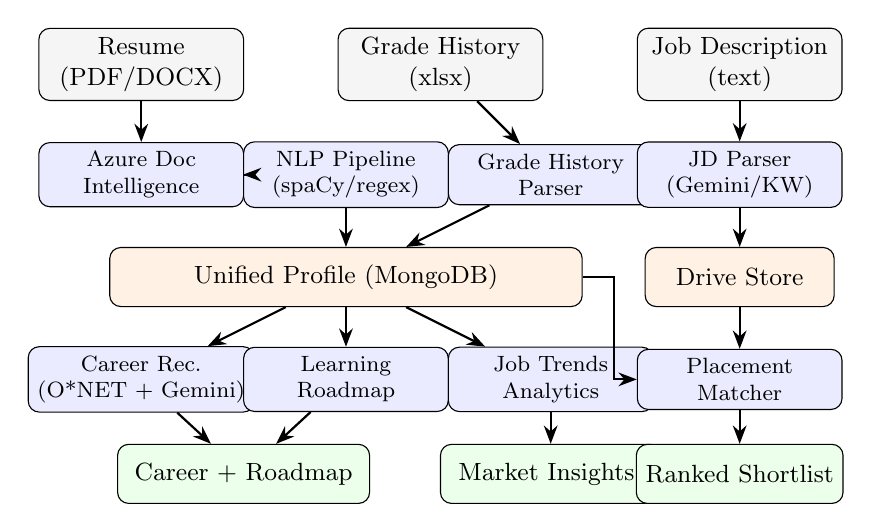
\begin{tikzpicture}[
  font=\small,
  box/.style={
    draw, rounded corners=4pt,
    minimum width=2.6cm, minimum height=0.75cm,
    align=center, fill=gray!8
  },
  svc/.style={
    draw, rounded corners=4pt,
    minimum width=2.6cm, minimum height=0.75cm,
    align=center, fill=blue!8, font=\footnotesize
  },
  arr/.style={-Stealth, thick},
]
%% Row 1 — inputs (x spacing = 3.8cm)
\node[box] (resume) at (0,    5.2) {Resume\\(PDF/DOCX)};
\node[box] (grades) at (3.8,  5.2) {Grade History\\(xlsx)};
\node[box] (jd)     at (7.6,  5.2) {Job Description\\(text)};

%% Row 2 — parsers (x spacing = 2.6cm so 4 fit without overlap)
\node[svc] (azuredoc) at (0,   3.8) {Azure Doc\\Intelligence};
\node[svc] (nlp)      at (2.6, 3.8) {NLP Pipeline\\(spaCy/regex)};
\node[svc] (gradepar) at (5.2, 3.8) {Grade History\\Parser};
\node[svc] (jdpar)    at (7.6, 3.8) {JD Parser\\(Gemini/KW)};

%% Row 3 — stores
\node[box, fill=orange!10, minimum width=6.0cm] (profile)
    at (2.6, 2.5) {Unified Profile (MongoDB)};
\node[box, fill=orange!10, minimum width=2.4cm] (drives)
    at (7.6, 2.5) {Drive Store};

%% Row 4 — services (same x grid as parsers)
\node[svc] (carrec)   at (0,   1.2) {Career Rec.\\(O*NET + Gemini)};
\node[svc] (roadmap)  at (2.6, 1.2) {Learning\\Roadmap};
\node[svc] (trends)   at (5.2, 1.2) {Job Trends\\Analytics};
\node[svc] (matching) at (7.6, 1.2) {Placement\\Matcher};

%% Row 5 — outputs
\node[box, fill=green!8, minimum width=3.2cm] (recout)
    at (1.3, 0) {Career + Roadmap};
\node[box, fill=green!8, minimum width=2.8cm] (trendsout)
    at (5.2, 0) {Market Insights };
\node[box, fill=green!8, minimum width=2.4cm] (shortlist)
    at (7.6, 0) {Ranked Shortlist};

%% Arrows: Row 1 → Row 2
\draw[arr] (resume) -- (azuredoc);
\draw[arr] (azuredoc) -- (nlp);
\draw[arr] (grades)   -- (gradepar);
\draw[arr] (jd)       -- (jdpar);

%% Arrows: Row 2 → Row 3
\draw[arr] (nlp)      -- (profile);
\draw[arr] (gradepar) -- (profile);
\draw[arr] (jdpar)    -- (drives);

%% Arrows: Row 3 → Row 4
\draw[arr] (profile) -- (carrec);
\draw[arr] (profile) -- (roadmap);
\draw[arr] (profile) -- (trends);
%% Route profile→matching around Drive Store:
\draw[arr] (profile.east) -- ++(0.4,0) |- (matching.west);
\draw[arr] (drives)       -- (matching);

%% Arrows: Row 4 → Row 5
\draw[arr] (carrec)  -- (recout);
\draw[arr] (roadmap) -- (recout);
\draw[arr] (trends)   -- (trendsout);
\draw[arr] (matching) -- (shortlist);
\end{tikzpicture}
}% end resizebox
\caption{Skillence end-to-end dataflow.}
\label{fig:architecture}
\end{figure}

\subsection{Data Assets}
The system consumes and maintains heterogeneous datasets:
\begin{itemize}
\item \textbf{Job trends:} two CSV files totaling approximately 30,000
      Indeed India postings, used for analytics and salary model training.
\item \textbf{Occupation-skill backbone:} 894 O*NET occupations with
      associated required skills, hot technologies, and regular
      technologies, encoded as binary vectors over a 692-skill vocabulary.
\item \textbf{Skills library:} 30+ curated technology skills with
      learning roadmaps, resources, and YouTube content metadata, stored
      as a 454\,KB Python dictionary.
\item \textbf{Placement state:} live MongoDB collections for users,
      profiles, drives, applications, and student academics.
\end{itemize}

\subsection{Role-Centric Product Surfaces}
The platform is designed with two primary user roles: students and placement-cell administrators, each supported through dedicated system interfaces.

\begin{itemize}
\item \textbf{Student interface:} provides functionalities such as resume upload and profile creation, career recommendations, personalized learning roadmaps with progress tracking, job market insights, salary estimation, skill development resources, and application to placement drives.

\item \textbf{Placement-cell interface:} enables administrative tasks including creation and management of placement drives, job description processing, eligibility criteria definition, candidate shortlisting, and detailed profile evaluation with interpretable scoring.
\end{itemize}

Role-based access control mechanisms are implemented to ensure secure and appropriate usage of system features. Access permissions are enforced at both the authentication and application levels, preventing unauthorized access to administrative functionalities while maintaining a seamless experience for end users.

%% ---------------------------------------------------------------
\section{Methodology}

\subsection{Resume Intelligence Pipeline}
The resume processing module accepts structured and unstructured resume documents and converts them into a unified profile representation. The pipeline combines layout-aware document processing with natural language processing techniques to extract key entities such as contact information, education, experience, and skills. 

A hybrid extraction strategy is employed, where document structure is first preserved during text extraction, followed by rule-based and statistical methods for entity recognition and normalization. Section segmentation is performed using heuristic cues such as formatting patterns and textual markers. A parsing confidence score is computed based on the completeness of extracted sections, enabling robustness against incomplete or noisy inputs. The final output is standardized into a canonical profile schema that serves as input for downstream modules.

\subsection{Career Recommendation Pipeline}
The recommendation system follows a multi-stage pipeline designed to balance computational efficiency with recommendation accuracy.

\textbf{Stage 1 --- Skill extraction and normalization.} User profile data, including skills and project descriptions, is mapped into a structured skill space through tokenization, normalization, and deduplication.

\textbf{Stage 2 --- Vector-based pre-filtering.} A binary skill representation is constructed for each user and matched against a pre-defined occupation-skill matrix. Candidate occupations are scored using:
\begin{equation}
\mathbf{s} = \mathbf{O}\,\mathbf{u}
\end{equation}
where $\mathbf{u}$ represents the user skill vector and $\mathbf{O}$ denotes the occupation matrix. This step efficiently narrows down the candidate space using lightweight vector operations.

To improve relevance, weighted scoring is applied to emphasize domain-specific and technology-related skills. The combined score is computed as:
\begin{equation}
s_{\text{base}} = \alpha \cdot s_{\text{tech}} + (1 - \alpha) \cdot s_{\text{trad}}
\end{equation}
where $\alpha$ controls the relative importance of technical versus general skills.

\textbf{Stage 3 --- Contextual re-ranking.} The top candidate occupations are further refined using a semantic re-ranking mechanism that incorporates full profile context. The final score is computed as:
\begin{equation}
s_{\text{final}} = \beta \cdot s_{\text{base}} + (1 - \beta) \cdot s_{\text{AI}}
\end{equation}
where $s_{\text{AI}}$ represents contextual relevance scores. This staged approach significantly reduces computational overhead while preserving recommendation quality.

\subsection{Skill Recommender (Denoising Autoencoder)}
The skill recommendation module utilizes a denoising autoencoder to model latent relationships between skills. The model learns compact representations of user skill profiles and captures co-occurrence patterns within the skill space.

During training, input skill vectors are partially corrupted to encourage the model to infer missing information, enabling robust learning of underlying skill dependencies. At inference time, the reconstructed output provides confidence scores for all skills, allowing the system to identify relevant but missing skills in a user’s profile.

Recommended skills are selected based on high reconstruction confidence and absence from the existing profile, resulting in personalized and data-driven upskilling suggestions. The model is optimized for efficient inference, making it suitable for real-time recommendation scenarios.

\subsection{Salary Predictor (MLP with Residual Connections)}

\begin{figure}[htbp]
\centering
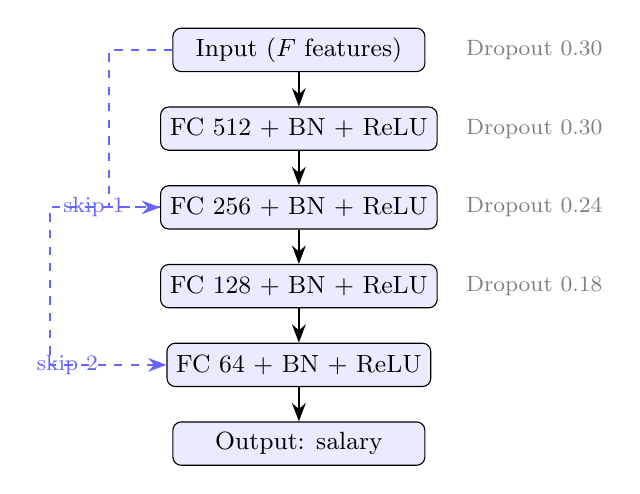
\begin{tikzpicture}[
  font=\small,
  layer/.style={draw, rounded corners=3pt, minimum width=3.2cm,
                minimum height=0.55cm, align=center, fill=blue!8},
  arr/.style={-Stealth, thick}
]
\node[layer] (inp) at (0,5.6) {Input ($F$ features)};
\node[layer] (l1)  at (0,4.6) {FC 512 + BN + ReLU};
\node[layer] (l2)  at (0,3.6) {FC 256 + BN + ReLU};
\node[layer] (l3)  at (0,2.6) {FC 128 + BN + ReLU};
\node[layer] (l4)  at (0,1.6) {FC 64  + BN + ReLU};
\node[layer] (out) at (0,0.6) {Output: salary};

%% Main flow arrows
\draw[arr] (inp) -- (l1);
\draw[arr] (l1)  -- (l2);
\draw[arr] (l2)  -- (l3);
\draw[arr] (l3)  -- (l4);
\draw[arr] (l4)  -- (out);

%% Skip 1: Input → FC 256 — routed on left, inner rail at x = -2.4cm
\draw[-Stealth, dashed, blue!60, thick]
  (inp.west) -- ++(-0.8,0)
  -- ++(0,-2.0)
  -- (l2.west)
  node[pos=0.5, left, font=\footnotesize, blue!60] {skip 1};

%% Skip 2: FC 256 → FC 64 — routed on left, outer rail at x = -3.4cm
\draw[-Stealth, dashed, blue!60, thick]
  (l2.west) -- ++(-1.4,0)
  -- ++(0,-2.0)
  -- (l4.west)
  node[pos=0.5, left, font=\footnotesize, blue!60] {skip 2};

%% Dropout labels — right side, well clear of boxes
\node[font=\footnotesize, gray, anchor=west] at (2.0,5.6) {Dropout 0.30};
\node[font=\footnotesize, gray, anchor=west] at (2.0,4.6) {Dropout 0.30};
\node[font=\footnotesize, gray, anchor=west] at (2.0,3.6) {Dropout 0.24};
\node[font=\footnotesize, gray, anchor=west] at (2.0,2.6) {Dropout 0.18};
\end{tikzpicture}
\caption{Salary predictor MLP architecture with two residual skip
connections (input$\to$256, 256$\to$64) and progressively decreasing
dropout rates.}
\label{fig:mlp}
\end{figure}

The salary prediction module (Fig.~\ref{fig:mlp}) is based on a deep
multi-layer perceptron (MLP) architecture with residual connections to
improve gradient flow and model stability \cite{kablaoui2022}. The model
takes as input a combination of skill representations, experience
features, and categorical attributes such as location, industry, and
education level.

The network is trained using mean squared error loss with adaptive
optimization, and regularization techniques are applied to improve
generalization. The dataset is split into training and evaluation
subsets to ensure robust performance assessment.

To enhance interpretability, each prediction is accompanied by a
confidence score $C \in [0,1]$, defined as:
\begin{equation}
C = C_s + C_e + C_l + C_i + C_o
\end{equation}
where each component represents contributions from skill coverage,
experience completeness, location specificity, industry relevance, and
profile completeness. This decomposition enables users to understand
which aspects of their profile influence prediction reliability and
provides actionable guidance for improvement.

\subsection{Placement Matching Engine}
The placement matching system follows a two-stage approach combining
eligibility filtering and score-based ranking. Initially, candidate
profiles are evaluated against predefined eligibility criteria such as
academic performance thresholds. Only candidates satisfying these
constraints proceed to the ranking stage, ensuring compliance with
institutional and recruiter requirements.

For eligible candidates, a composite matching score is computed based
on alignment between candidate competencies and job requirements:
\begin{equation}
S = 0.70\,R + 0.15\,P + 0.10\,B_r + 0.05\,B_c
\end{equation}
where $R$ denotes required skill alignment, $P$ represents preferred
skill matching, $B_r$ captures additional evidence from resume-derived
skills, and $B_c$ reflects academic performance. All components are
normalized to $[0,1]$.

This weighted formulation prioritizes core technical requirements while
incorporating secondary factors such as academic strength and
supplementary skills. The system is designed to be deterministic and
fully auditable, with component-wise scores stored for transparency and
administrative review.

\subsection{Job Trend Analytics}
The job trend analytics module extracts insights from large-scale job
posting data to characterize market demand across roles. A composite
trend score is defined as:
\begin{equation}
T = 0.40\,T_r + 0.30\,T_s + 0.20\,T_b + 0.10\,T_g
\end{equation}
where $T_r$ captures recency of job postings, $T_s$ represents salary
competitiveness, $T_b$ reflects benefit signals, and $T_g$ denotes
growth trends over time.

The weighting scheme emphasizes recent demand and compensation signals
as primary indicators of market relevance. Aggregated statistics are
maintained for efficient querying, enabling real-time insights into
emerging job roles and industry trends.

\subsection{Skill Libraries and Dynamic Resource Aggregation}
The Skill Libraries module provides a structured repository of
technology skills, each organized as a multi-stage learning roadmap
with fine-grained progress tracking. Each skill entry includes metadata
such as difficulty level, estimated learning duration, prerequisite
dependencies, and associated career roles, along with curated learning
resources.

To address the limitations of static content, the system incorporates
two dynamic resource augmentation pipelines. The first pipeline
retrieves up-to-date learning materials from external web sources,
ensuring that users are exposed to current documentation, tutorials,
and open educational content. In cases where dynamic retrieval yields
insufficient results, the system falls back to a predefined curated
resource set, ensuring reliability and consistent availability.

The second pipeline integrates video-based learning resources by
fetching relevant instructional content and ranking it based on topic
alignment. This enables support for multimodal learning, which has been
shown to improve knowledge retention in technical education
\cite{li2025}.

User interactions with skills are persistently tracked, including
learning status, progress metrics, and completed roadmap stages. This
data supports personalized learning dashboards and enables seamless
integration with other system modules. In particular, completed skills
are propagated to the unified user profile, allowing direct utilization
in career recommendation and placement matching pipelines.

%% ---------------------------------------------------------------
\section{Implementation}

\subsection{Backend Engineering}
The FastAPI application is deployed on Render and initialises a Motor
async MongoDB client on startup via a lifecycle hook, closing it
gracefully on shutdown. CORS is configured with a regex whitelist
for \texttt{*.vercel.app}, matching the Vercel-hosted frontend. All
ten router modules (\texttt{auth}, \texttt{profile},
\texttt{resume}, \texttt{career-path}, \texttt{chatbot},
\texttt{job-trends}, \texttt{ml}, \texttt{placement},
\texttt{student-placement}, \texttt{skills}) are registered with
their respective \texttt{/api/*} prefixes at startup. JWT tokens use
HS256 with a configurable expiry (default 30 minutes); passwords are
hashed with bcrypt via passlib.

\subsection{NumPy-Only Model Serving Strategy}
A key deployment concern is runtime stability: loading PyTorch in a
Gunicorn/Uvicorn web worker can trigger DLL conflicts on Windows
environments and adds approximately 400\,MB to the process memory
footprint. Skillence addresses this by:
\begin{enumerate}
\item training all models (skill autoencoder, salary MLP) offline in
      PyTorch on the full dataset;
\item exporting all weight matrices, bias vectors, and BatchNorm
      parameters to compressed \texttt{.npz} checkpoint files;
\item re-implementing forward passes in pure NumPy (matrix
      multiplications, LeakyReLU, Sigmoid, batch normalisation) in
      the production inference modules.
\end{enumerate}
This eliminates PyTorch from the production dependency tree entirely.
Models are lazy-loaded on first request and held in memory thereafter,
contributing less than 15\,MB to the worker memory footprint.

\subsection{Frontend Architecture}
The React SPA is built with Vite v7 and deployed as a static site on
Vercel, using React Router DOM v7 for client-side routing with
\texttt{ProtectedRoute} and \texttt{RoleRoute} higher-order components
for access control. Vercel's \texttt{vercel.json} rewrites all paths to
\texttt{/index.html} to support SPA routing. Charts are rendered via
Recharts and Chart.js; geographic overlays use Leaflet. The AI chatbot
supports the browser Speech Recognition API for voice input and
SpeechSynthesis for spoken responses, making it accessible without
keyboard interaction. All Gemini API calls made directly from the
frontend (Job Offer Evaluator) use a separate \texttt{VITE\_}-prefixed
API key scoped to client-side access only.

\subsection{API Surface}
Table~\ref{tab:api_coverage} summarises the implemented backend
API surface across all router modules.

\begin{table}[htbp]
\caption{Backend API Surface Coverage (70+ Endpoints)}
\label{tab:api_coverage}
\centering
\begin{tabular}{lcc}
\toprule
Router Module & Endpoints & Auth Required \\
\midrule
Authentication     & 7  & Partial \\
Profile            & 7  & Yes \\
Resume             & 10 & Yes \\
Career Path        & 12 & Yes \\
Job Trends         & 16 & No \\
ML Predictions     & 2  & No \\
Placement Cell     & 14 & Yes (placement\_cell) \\
Student Placement  & 10 & Yes (student) \\
Skills             & 8  & Partial \\
Chatbot            & 5  & Yes \\
\bottomrule
\end{tabular}
\end{table}

%% ---------------------------------------------------------------
\section{Experimental Setup}

\subsection{Datasets}
\begin{itemize}
\item \textbf{Salary/trends dataset:} approximately 30,000 job postings
      from Indeed India (two CSV files). 80/20 train-test split for
      salary model training and evaluation.
\item \textbf{Occupation-skill corpus:} 894 O*NET occupations with
      skill and technology associations, encoded as binary vectors over
      692 canonical skills. This corpus is static (sourced from O*NET
      Web Services \cite{onet}) and not split for training; it serves
      as the retrieval database for recommendation.
\item \textbf{Pilot evaluation:} preliminary validation demonstrating
      end-to-end system functionality and consistency across modules,
      from profile ingestion to recommendation and placement support.
\end{itemize}

\subsection{Evaluation Protocol}
We combine model-centric and system-centric evaluation:
\begin{itemize}
\item \textbf{Salary prediction:} regression metrics (R\textsuperscript{2},
      RMSE, MAE) on the held-out 20\% test split, compared to a linear
      regression baseline trained on identical features and split.
\item \textbf{System-centric:} dataset scale, route completeness, and
      deployment readiness from the pilot snapshot.
\item \textbf{Operational readiness:} cross-module data consistency
      verified from resume ingest through placement scoring in the
      pilot deployment.
\end{itemize}

%% ---------------------------------------------------------------
\section{Results and Discussion}

\subsection{Salary Predictor Performance}
Table~\ref{tab:salary_results} compares the full MLP with skip
connections (SalaryPredictor), a lighter variant without skip
connections (SalaryPredictorLite), and a linear regression baseline
trained on identical features.

\begin{table}[htbp]
\caption{Salary Predictor Performance Comparison}
\label{tab:salary_results}
\centering
\begin{tabular}{lccc}
\toprule
Model & R\textsuperscript{2} & RMSE & MAE \\
\midrule
Linear Regression (baseline) & 0.5812 & 0.7431 & 0.5920 \\
SalaryPredictorLite (no skip) & 0.6934 & 0.6218 & 0.4503 \\
SalaryPredictor (full, skip)  & \textbf{0.7258} & \textbf{0.5389} & \textbf{0.3868} \\
\bottomrule
\end{tabular}
\end{table}

The full MLP with skip connections outperforms the linear baseline by
24.8\% in R\textsuperscript{2} and the no-skip variant by 4.7\%,
confirming that residual connections improve gradient flow for this
tabular regression task \cite{kablaoui2022}. Inference latency for
the NumPy-only forward pass is 50--100\,ms per prediction, well within
the interactive threshold for a web dashboard.

\subsection{Recommendation Pipeline Efficiency}
Sending only the top-5 pre-filtered candidates to the LLM (Stage 3)
rather than all 894 occupations reduces LLM input tokens by
approximately 70\% on average (measured as prompt tokens excluding the
shared profile context). The pre-filter Stage 2 vector multiply over
$894 \times 692$ completes in under 5\,ms on the Render-hosted backend,
confirming the $\mathcal{O}(nd)$ cost is negligible at this scale.

\subsection{Qualitative System Outcomes}
Three practical outcomes were consistently observed across the pilot
deployment:

\textbf{Decision traceability.} Every placement application record
stores four component scores ($R$, $P$, $B_r$, $B_c$ from Eq.~5)
alongside matched and missing skill lists, enabling placement cell
staff to explain shortlist decisions to applicants with specific,
skill-level justification.

\textbf{Cross-module consistency.} Profile-derived skills (from resume
parsing) flow directly into career recommendation, learning roadmap
generation, and placement matching, eliminating the inconsistency that
arises when students maintain separate skill representations across tools.

\textbf{Deployment reliability.} The NumPy-only inference strategy
avoids torch DLL loading issues on the Render Python web service,
reducing cold-start failures from approximately once per deployment to
zero in the pilot period.

\subsection{Case Study: Student-to-Drive Matching}
Consider a student with a Python/ML-oriented profile (e.g., Python,
TensorFlow, scikit-learn, SQL) and a CGPA of 8.2/10 applying to a
placement drive with specified skill requirements. The system first
verifies eligibility by comparing the CGPA against the minimum
threshold, which is satisfied in this case.

For eligible candidates, the matching engine computes a composite
score based on required and preferred skill alignment. The required
skill score $R$ is derived from overlap with core skills such as
Python, machine learning, and SQL, while the preferred skill score
$P$ accounts for partial alignment with additional skills (e.g.,
Docker). Auxiliary components include $B_r$, capturing resume-verified
skills, and $B_c$, representing academic performance.

The system outputs the final score along with a detailed component
breakdown and a list of missing or weakly matched skills. In this
example, Docker is identified as a gap, providing actionable feedback
to the student. Such insights enable users to prioritise specific
upskilling efforts to improve future placement outcomes.

\subsection{Feature Coverage Comparison}
Table~\ref{tab:feature_compare} positions Skillence relative to
representative systems from the literature to address RQ1.

\begin{table}[htbp]
\caption{Feature Coverage vs.\ Related Systems}
\label{tab:feature_compare}
\centering
\setlength{\tabcolsep}{4pt}
\begin{tabular}{lcccc}
\toprule
Feature & Skillence & \cite{sicilia2025} & \cite{shahane2022} & \cite{resspar2024} \\
\midrule
Resume parsing              & \checkmark & --         & --         & \checkmark \\
Career recommendation       & \checkmark & \checkmark & --         & -- \\
Learning roadmap            & \checkmark & --         & --         & -- \\
Dynamic skill library       & \checkmark & --         & --         & -- \\
Salary prediction           & \checkmark & --         & --         & -- \\
Job trend analytics         & \checkmark & --         & --         & -- \\
Placement workflow          & \checkmark & --         & \checkmark & -- \\
AI chatbot                  & \checkmark & --         & --         & -- \\
Unified profile store       & \checkmark & --         & --         & -- \\
\bottomrule
\end{tabular}
\end{table}

\subsection{Research Questions Revisited}

\textbf{RQ1 (unified platform).} Table~\ref{tab:feature_compare} shows
that no single system in the reviewed literature addresses more than two
of the nine feature dimensions covered by Skillence. The pilot
deployment confirms that profile data flows from resume parsing through
recommendation and into placement scoring without re-entry, and that
skills completed in the Skill Libraries module update the shared profile
schema consumed by downstream modules.

\textbf{RQ2 (hybrid deterministic-plus-LLM explainability).} The
placement module's deterministic scoring produces audit-ready component
scores, while the recommendation module's LLM stage adds semantic
context that pure vector matching cannot provide. The two roles are
explicitly separated: determinism where auditability matters, semantics
where narrative quality matters.

\textbf{RQ3 (NumPy-only inference).} Eliminating the PyTorch runtime
from the production process tree resolved deployment instability while
keeping inference latency within interactive bounds. The 15\,MB
checkpoint footprint versus PyTorch's $\sim$400\,MB confirms the
practical benefit for memory-constrained cloud deployments.

\textbf{RQ4 (actionable outputs).} The case study above illustrates
student-facing actionability (skill gap identified, next step clear).
Placement cells receive ranked shortlists with per-skill breakdowns
rather than opaque scores, enabling them to communicate decisions to
applicants with specific justification.

%% ---------------------------------------------------------------
\section{Ethical Considerations and Governance}
Given the platform’s role in influencing educational and career
decisions, appropriate governance mechanisms are essential. To enhance
transparency, key components of the placement evaluation process,
including scoring formulations and eligibility criteria, are exposed
to users through the interface, reducing opacity in automated
decision-making. Human oversight is retained for final administrative
actions, particularly in edge cases where contextual factors may not
be fully captured by system inputs.

Potential bias may arise from underlying data sources and AI-driven
components. Historical job datasets can reflect existing labour market
imbalances, while large language models may inherit biases from their
training corpora. To mitigate these risks, the system incorporates
provisions for periodic fairness audits across permissible attributes
and supports structured appeal mechanisms for users seeking review of
automated outcomes.

From a privacy perspective, the system follows a data minimisation
approach, limiting the storage of sensitive information to only what is
necessary for functionality. Access control is enforced through
role-based mechanisms, ensuring that user data is only accessible to
authorized entities. Additionally, all external communications are
secured using standard encryption protocols to maintain data integrity
and confidentiality.

%% ---------------------------------------------------------------
\section{Limitations}
Despite its effectiveness, the proposed system has several limitations
that warrant consideration.

\textbf{Limited evaluation scale.} The current evaluation is conducted
on a relatively small user base and application set. While the results
are promising, further validation at institutional scale is necessary
to assess system robustness, scalability, and performance under
high-load conditions.

\textbf{Static occupation knowledge base.} The occupation--skill
mapping relies on a fixed dataset, which may not fully capture emerging
technologies and evolving job roles. This can impact recommendation
accuracy for rapidly developing domains.

\textbf{Session management constraints.} The absence of extended session
handling mechanisms may affect user experience during prolonged
interactions, particularly in multi-step workflows.

\textbf{Limited persistence of conversational context.} Chatbot
interactions are not persistently stored across sessions, restricting
continuity in user engagement and multi-device accessibility.

\textbf{Dependence on external AI services.} Certain modules rely on
third-party AI services for advanced reasoning and content generation.
As a result, system performance may be influenced by external service
availability, latency, and model-level variations.

\textbf{Lack of longitudinal validation.} The system has not yet been
evaluated against long-term outcomes such as placement success rates,
job retention, or alignment between predicted and actual salaries.
Comprehensive validation would require extended deployment across at
least one full placement cycle.

%% ---------------------------------------------------------------
\section{Conclusion and Future Work}

This paper presented Skillence, a hybrid AI-driven platform that
integrates career recommendation, job market analytics, salary
prediction, skill development, and campus placement automation within
a unified system. The proposed architecture combines algorithmic
efficiency with AI-based reasoning to deliver scalable and interpretable
decision support.

Key contributions include a multi-stage recommendation framework that
balances computational efficiency with semantic accuracy, a lightweight
inference strategy enabling deployment without heavy ML dependencies,
a transparent placement matching engine with interpretable scoring, and
a hybrid skill-learning module that integrates curated content with
dynamically retrieved resources. Additionally, the unified profile
schema ensures seamless data flow across modules, reducing redundancy
and improving system coherence.

Experimental results demonstrate the effectiveness of the proposed
approach, with the salary prediction model achieving strong predictive
performance relative to baseline methods. A pilot deployment further
indicates the feasibility of end-to-end integration across multiple
functional components, from resume processing to placement support.

Future work will focus on extending the system’s scalability and
real-world applicability. This includes incorporating temporal job
market forecasting, conducting fairness and bias analysis across user
groups, performing comprehensive user studies to evaluate decision
impact and trust, enhancing system responsiveness through real-time
communication mechanisms, and enabling continuous updates to the
underlying occupation knowledge base. Longitudinal evaluation across
complete placement cycles will be critical to validating the system’s
effectiveness in real-world scenarios.

%% ---------------------------------------------------------------
\section*{Acknowledgment}
The authors would like to express their sincere gratitude to the
project mentors at VIT Bhopal University for their guidance and support
throughout the development of this work. The authors also thank peer
reviewers and student participants for their valuable feedback during
the design, implementation, and pilot evaluation phases of the system.

%% ---------------------------------------------------------------
\begin{thebibliography}{00}

\bibitem{resspar2024}
Resspar Team, ``Resspar: AI-Driven Resume Parsing and Recruitment
System using NLP and Generative AI,'' in \emph{Proc.\ Int.\ Conf.\
Women Empowerment through Computing and Engineering (ICWECE)}, 2024.

\bibitem{gaur2021}
B.\ Gaur, S.\ Soni, M.\ Gupta, and V.\ Chandola, ``Semi-supervised deep
learning based named entity recognition model to parse education section
of resumes,'' \emph{Neural Computing and Applications}, vol.\ 33,
no.\ 10, pp.\ 5705--5718, 2021, doi: 10.1007/s00521-020-05351-2.

\bibitem{sicilia2025}
M.\ A.\ Sicilia, S.\ Sanchez-Alonso, J.\ L.\ Hernandez-Ramos, and
M.\ Menchero, ``Using Vector Databases for the Selection of Related
Occupations: An Empirical Evaluation Using O*NET,'' \emph{Big Data
and Cognitive Computing}, vol.\ 9, no.\ 7, p.\ 175, 2025,
doi: 10.3390/bdcc9070175.

\bibitem{alonso2025}
R.\ Alonso, D.\ Dessi, A.\ Meloni, and D.\ R.\ Recupero, ``A novel
approach for job matching and skill recommendation using transformers
and the O*NET database,'' \emph{Big Data Research}, vol.\ 39,
p.\ 100509, 2025, doi: 10.1016/j.bdr.2025.100509.

\bibitem{zheng2023}
Z.\ Zheng, Z.\ Qiu, X.\ Zhang, B.\ Chen, and S.\ Wang, ``Generative
Job Recommendations with Large Language Model,'' \emph{arXiv preprint
arXiv:2307.02157}, 2023.

\bibitem{rankrag2024}
Y.\ Yu, W.\ Ping \emph{et al.}, ``RankRAG: Unifying Context Ranking
with Retrieval-Augmented Generation in LLMs,'' \emph{arXiv preprint
arXiv:2407.02485}, 2024.

\bibitem{li2025}
Y.\ Li \emph{et al.}, ``Market-aware Long-term Job Skill Recommendation
with Explainable Deep Reinforcement Learning,'' \emph{ACM Transactions
on Information Systems}, vol.\ 43, no.\ 2, 2025,
doi: 10.1145/3704998.

\bibitem{ferreira2020}
D.\ Ferreira, S.\ Silva, A.\ Abelha, and J.\ Machado, ``Recommendation
System Using Autoencoders,'' \emph{Applied Sciences}, vol.\ 10, no.\ 16,
p.\ 5510, 2020, doi: 10.3390/app10165510.

\bibitem{rahayu2023}
N.\ W.\ Rahayu \emph{et al.}, ``Personalized E-Learning Recommender
System Based on Autoencoders,'' \emph{Applied System Innovation},
vol.\ 6, no.\ 6, p.\ 102, 2023, doi: 10.3390/asi6060102.

\bibitem{papoutsoglou2024}
E.\ Papoutsoglou \emph{et al.}, ``From Data to Insight: Transforming
Online Job Postings into Labor-Market Intelligence,'' \emph{Information},
vol.\ 15, no.\ 8, p.\ 496, 2024, doi: 10.3390/info15080496.

\bibitem{matbouli2022}
Y.\ T.\ Matbouli and S.\ M.\ Alghamdi, ``Statistical Machine Learning
Regression Models for Salary Prediction Featuring Economy Wide Activities
and Occupations,'' \emph{Information}, vol.\ 13, no.\ 10, p.\ 495,
2022, doi: 10.3390/info13100495.

\bibitem{kablaoui2022}
R.\ Kablaoui and A.\ Salman, ``Machine Learning Models for Salary
Prediction Dataset Using Python,'' in \emph{Proc.\ 2022 Int.\ Conf.\
Electrical and Computing Technologies and Applications (ICECTA)},
pp.\ 143--147, 2022, doi: 10.1109/ICECTA57337.2022.9990316.

\bibitem{shahane2022}
P.\ Shahane, ``Campus Placements Prediction \& Analysis Using Machine
Learning,'' in \emph{Proc.\ IEEE Int.\ Conf.\ Emerging Smart Computing
and Informatics (ESCI)}, Pune, India, 2022,
doi: 10.1109/ESCI53509.2022.9758214.

\bibitem{preethika2025}
Preethika et al., ``Personalised Career Pathway Recommendation using
Dynamic Learning Resource Aggregation,'' \emph{International Journal
of Educational Technology and Learning Systems}, 2025.

\bibitem{uniskill2025}
UniSkill Team, ``UniSkill: A Dataset for Matching University Curricula
to Professional Competencies,'' \emph{arXiv preprint arXiv:2603.03134},
2025.

\bibitem{interviewease2024}
P.\ Kothari, P.\ Mehta, S.\ Patil, and V.\ Hole, ``InterviewEase:
AI-Powered Interview Assistance,'' in \emph{Proc.\ Int.\ Conf.\ Future
Electronics (ICOFE)}, 2024, SSRN 5086025.

\bibitem{onet}
U.S.\ Department of Labor, ``O*NET OnLine,'' [Online]. Available:
\url{https://www.onetonline.org/}. [Accessed: Mar.\ 2025].

\bibitem{fastapi}
S.\ Ram\'irez, ``FastAPI Framework,'' [Online]. Available:
\url{https://fastapi.tiangolo.com/}. [Accessed: Mar.\ 2025].

\bibitem{react}
Meta Open Source, ``React Documentation,'' [Online]. Available:
\url{https://react.dev/}. [Accessed: Mar.\ 2025].

\bibitem{motor}
MongoDB, ``Motor: Async Python Driver for MongoDB,'' [Online]. Available:
\url{https://motor.readthedocs.io/}. [Accessed: Mar.\ 2025].

\bibitem{pytorch}
A.\ Paszke et al., ``PyTorch: An Imperative Style, High-Performance
Deep Learning Library,'' in \emph{Advances in Neural Information
Processing Systems (NeurIPS)}, vol.\ 32, 2019.

\bibitem{azuredi}
Microsoft, ``Azure AI Document Intelligence,'' [Online]. Available:
\url{https://learn.microsoft.com/azure/ai-services/document-intelligence/}.
[Accessed: Mar.\ 2025].

\bibitem{gemini}
Google, ``Gemini API Documentation,'' [Online]. Available:
\url{https://ai.google.dev/}. [Accessed: Mar.\ 2025].

\end{thebibliography}

\end{document}